\documentclass[tikz,border=10pt]{standalone}
\usepackage{tikz}
\usetikzlibrary{arrows.meta,positioning,shapes}
\usepackage{amsmath} % <<<<<<  AÑADIDO


\begin{document}

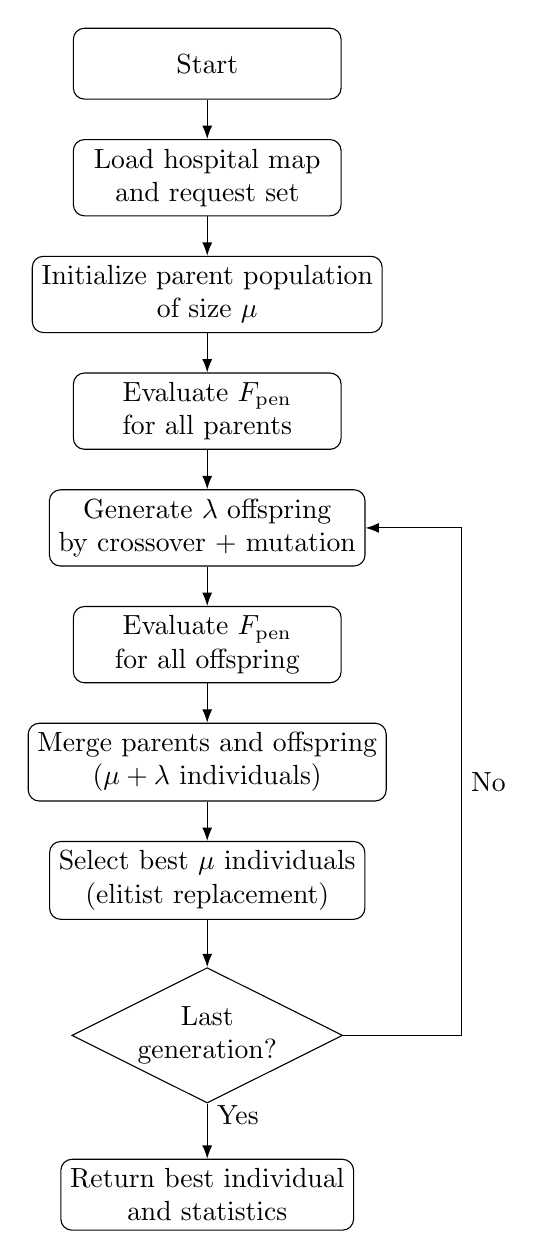
\begin{tikzpicture}[
  node distance=0.5cm,
  >=Latex,
  block/.style={rectangle, draw, rounded corners, align=center, minimum width=3.4cm, minimum height=0.9cm},
  decision/.style={diamond, draw, aspect=2, align=center, inner sep=1pt},
  line/.style={draw, -{Latex}}
]

\node[block] (start) {Start};
\node[block, below=of start] (env) {Load hospital map\\and request set};
\node[block, below=of env] (init) {Initialize parent population\\of size $\mu$};
\node[block, below=of init] (evalmu) {Evaluate $F_{\text{pen}}$\\for all parents};
\node[block, below=of evalmu] (offspring) {Generate $\lambda$ offspring\\by crossover + mutation};
\node[block, below=of offspring] (evaloff) {Evaluate $F_{\text{pen}}$\\for all offspring};
\node[block, below=of evaloff] (merge) {Merge parents and offspring\\($\mu+\lambda$ individuals)};
\node[block, below=of merge] (select) {Select best $\mu$ individuals\\(elitist replacement)};
\node[decision, below=of select, yshift=-0.1cm] (stop) {Last\\generation?};
\node[block, below=of stop, yshift=-0.2cm] (end) {Return best individual\\and statistics};

\path[line] (start) -- (env);
\path[line] (env) -- (init);
\path[line] (init) -- (evalmu);
\path[line] (evalmu) -- (offspring);
\path[line] (offspring) -- (evaloff);
\path[line] (evaloff) -- (merge);
\path[line] (merge) -- (select);
\path[line] (select) -- (stop);

\path[line] (stop.east) -- ++(1.5,0) |- (offspring.east) node[pos=0.25, right]{No};
\path[line] (stop.south) -- (end.north) node[pos=0.2, right]{Yes};

\end{tikzpicture}

\end{document}
